\part{Examples}
\section{Style testing}
\subsection*{General}
\begin{frame}[label=contents_sample]
  \frametitle{This is a slide deck just for testing}
  \mode<beamer>{
    \only<1>{\tableofcontents}
  }
  \only<2>{\tableofcontents[currentsection]}
\end{frame}

{\nologo
\begin{frame}[fragile]
  \frametitle{Interpolation in Python}
  Interpolation can be done using the SciPy interpolation submodule, e.g.:
  \begin{lstlisting}
from scipy.interpolate import interp1d
f = interp1d(xdata, ydata, kind='linear')
  \end{lstlisting}
  This creates a function object \lstinline|f| based on the given data.\pause
  \begin{columns}[T]
    \column{0.52\textwidth}
        \lstinputlisting[linerange={2-11}]{scripts/interpolation/demo-python-interp1d.py}
    \pause
      \lstinputlisting[linerange={13-13,17-18}]{scripts/interpolation/demo-python-interp1d.py}
      \pause
    \column{0.48\textwidth}
    \pause
      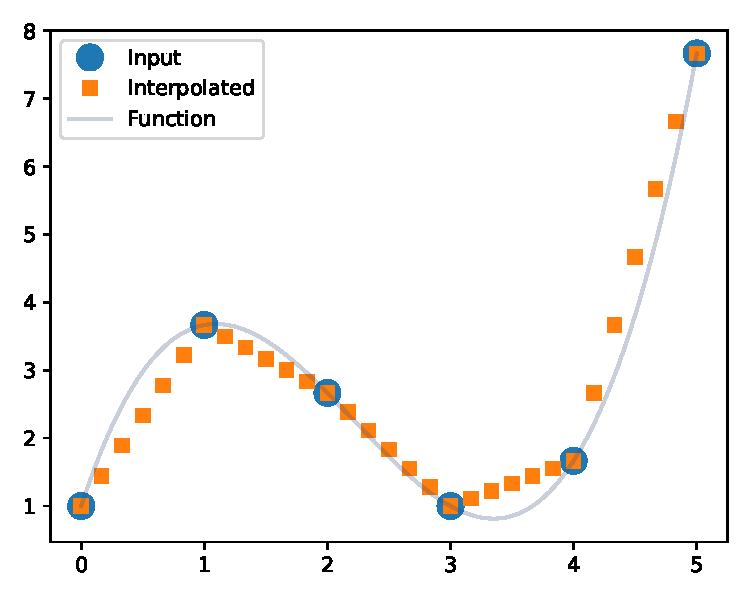
\includegraphics[width=0.9\textwidth]{demo-python-interp1d.pdf}
  \end{columns}
\end{frame}
}
